\documentclass[UTF8]{beamer}
\usepackage{ctex, hyperref}
\usepackage{fontspec}
\usepackage{latexsym,amsmath,xcolor,multicol,booktabs,calligra}
\usepackage{tikz}
\usepackage{graphicx,pstricks,listings,stackengine}
\usepackage{TJU}

\titlegraphic{
  
\includegraphics[height=2cm]{pic/QRCode.png}
}
\logo{
  \includegraphics[height=1cm]{pic/tjulogo.eps}
  % 
\includegraphics[height=0.9cm]{pic/QRCode.png}
}
\author{https://github.com/ChrisVicky/TJU-StudyAbroad}
\title{How to apply to Graduate Programs?}
\subtitle{-- a Guide with Example --}
\institute{College of Intelligence and Computing}
\date{\tiny \the\year.\the\month.\the\day}
% defs
\def\cmd#1{\texttt{\color{red}\footnotesize $\backslash$#1}}
\def\env#1{\texttt{\color{blue}\footnotesize #1}}
\definecolor{deepblue}{rgb}{0,0,0.5}
\definecolor{deepred}{rgb}{0.6,0,0}
\definecolor{deepgreen}{rgb}{0,0.5,0}
\definecolor{halfgray}{gray}{0.55}

\lstset{
  basicstyle=\ttfamily\small,
  keywordstyle=\bfseries\color{deepblue},
  emphstyle=\ttfamily\color{deepred},    % Custom highlighting style
  stringstyle=\color{deepgreen},
  numbers=left,
  numberstyle=\small\color{halfgray},
  rulesepcolor=\color{red!20!green!20!blue!20},
  frame=shadowbox,
}

\begin{document}

\begin{frame}
  \titlepage
\end{frame}


\begin{frame}
\begin{figure}
  \centering
  \tiny
  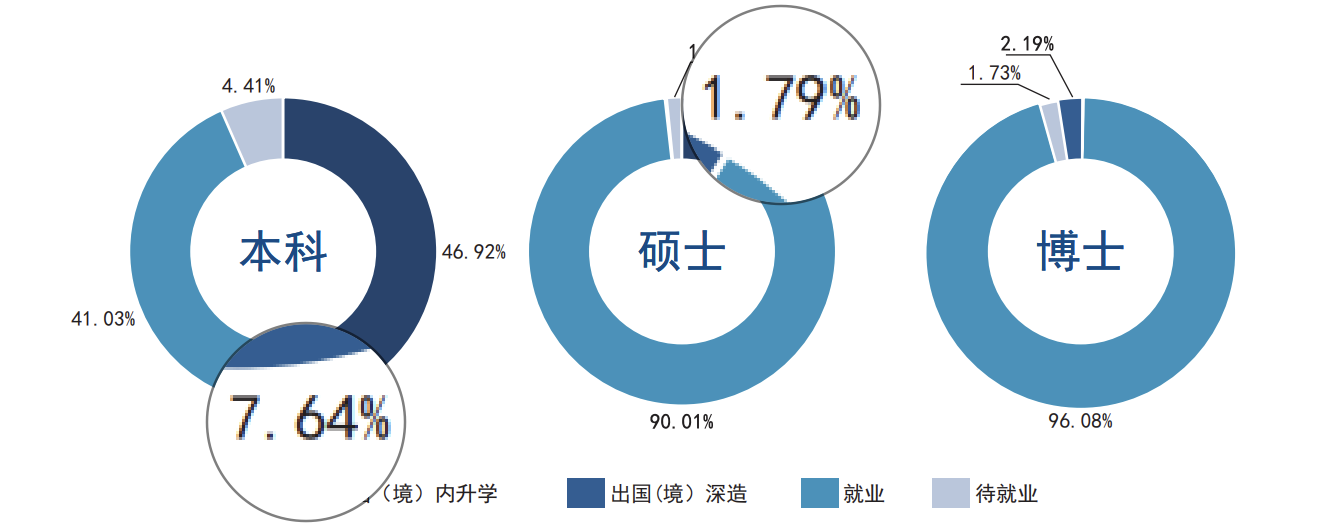
\includegraphics[width=.7\linewidth]{pic/2021-SA.png}
  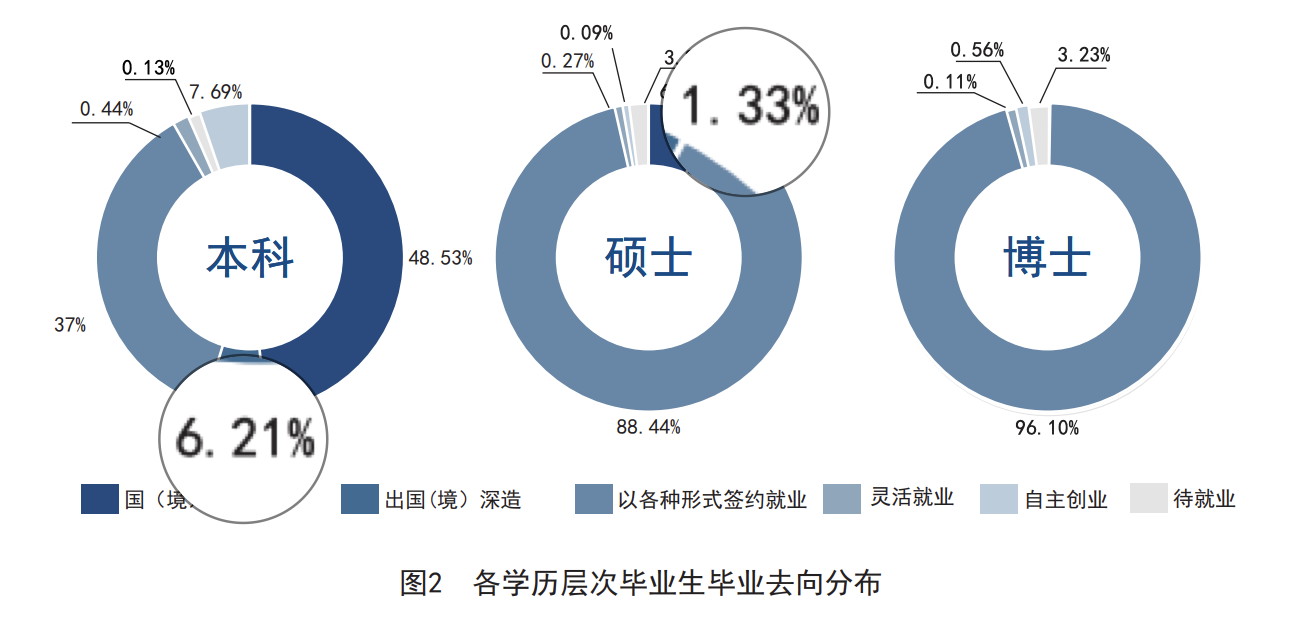
\includegraphics[width=.7\linewidth]{pic/2022-SA.png}
\end{figure}
{\tiny \noindent 2021: https://xxgkw.tju.edu.cn/xwgb1/202210/P020221028445708257318.pdf}

{\tiny \noindent 2022: https://xxgkw.tju.edu.cn/xwgb1/202310/P020231030586646916228.pdf}
\end{frame}


\begin{frame}
  \tableofcontents[sectionstyle=show,subsectionstyle=show/shaded/hide,subsubsectionstyle=show/shaded/hide]
\end{frame}



\section{How to Apply?}

\begin{frame}{\normalsize{Steps}}
  \begin{enumerate}

    \item Preparation: Information \& Planning

      \begin{itemize}
        \item Core Requirements: \hfill {\tiny GPA, TOEFL, Eligibility;}
        \item Additional Qualifications: \hfill {\tiny Research, Intern;}
        \item Timeline: \hfill {\tiny Exam, Deadlines;}
        \item Target Programs: \hfill {\tiny Research vs Course | T0, T1, T2;}
      \end{itemize}

    \item Actions
      \begin{itemize}
        \item Materials: \hfill {\tiny CV, SoI, Transcript;}
        \item Exams: \hfill {\tiny TOEFL, GRE;}
        \item Interviews: \hfill {\tiny Potential Supervisors, Committees;}
      \end{itemize}

    \item Harvest: Decision Making
      \begin{itemize}
        \item Offers: \hfill {\tiny Research vs Course Based;}
        \item Financials: \hfill {\tiny Scholarship vs Self-Fund;}
        \item Career Path: \hfill {\tiny Programs Courses, Alumni;}
      \end{itemize}
  \end{enumerate}
\end{frame}

\section{Examples}

\subsection{Information  \& Planning}
\begin{frame}{Where to look for Information? \hfill 2021.11 - 2022.11 \tiny{(Sophomore)}}
  \begin{itemize}
    \item Official Sites: e.g. \href{https://nusgs.nus.edu.sg/programmes-computing/}{\tiny{NUS Graduate School:} {\tiny https://nusgs.nus.edu.sg/programmes-computing/}}
    \item Keywords: Graduate Program + \$\{school\_name\}
  \end{itemize}
  \begin{figure}[h]
    \centering
    \includegraphics[width=\linewidth]{pic/SearchOnBaidu1.png}
  \end{figure}
\end{frame}

\begin{frame}{Planning \hfill 2021.11 - 2022.11 \tiny{(Sophomore)}}
  \begin{figure}[h]
    \centering
    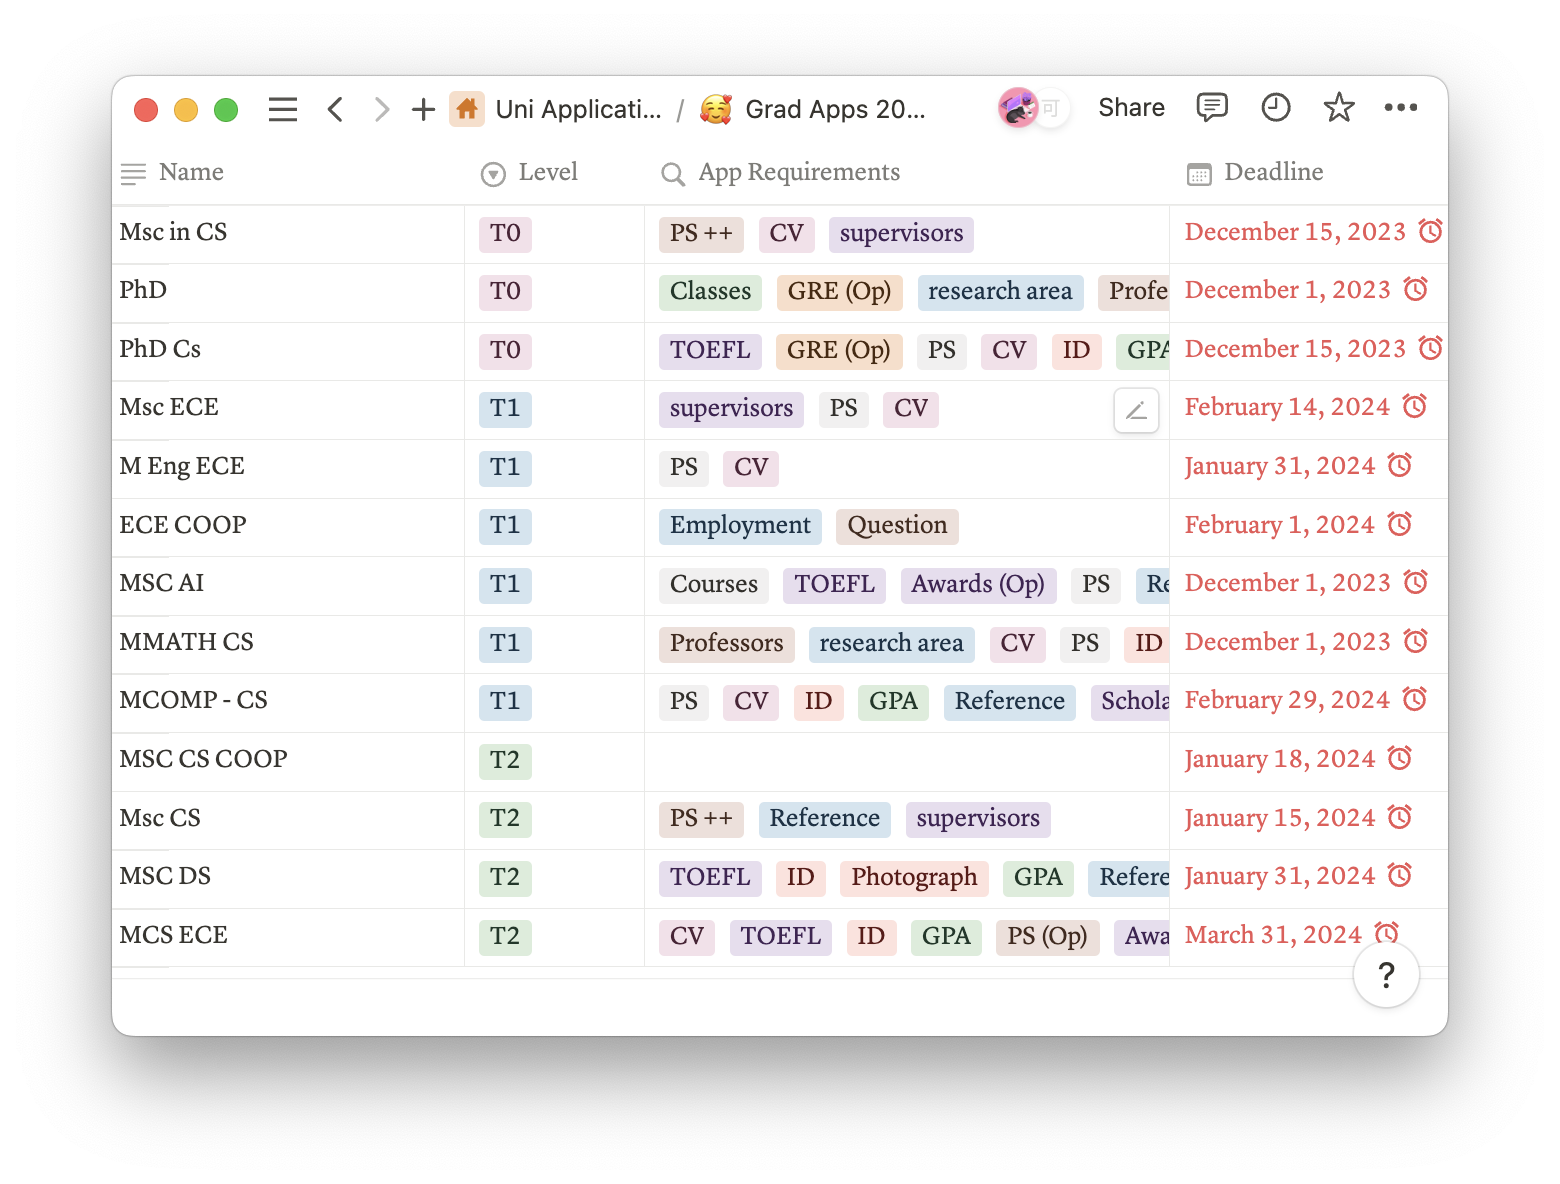
\includegraphics[width=.9\linewidth]{pic/SchoolList2.png}
  \end{figure}
\end{frame}

\subsection{Action Timeline}
\begin{frame}{Materials Preparation \hfill 2021.09 - 2023.09 \tiny{(Junior)}}
  \begin{itemize}
    \item Research: Join Labs \hfill 2021.09 - Now
    \item CV: Curriculum Vitae \hfill 2023.09 - 2023.11
    \item SoI: State of Interest \hfill 2023.09 - 2023.11
    \item Transcript: Maintain GPA \hfill -
    \item TOEFL   \hfill 2022.11 - 2023.01
  \end{itemize}
\end{frame}

\begin{frame}{Apply \hfill 2023.10 - 2024.02 \tiny{(Senior)}}
  \begin{itemize}
    \item Potential Supervisors \hfill 2023.10 - 2023.12
    \item Submit T0 \hfill 2023.12
    \item Submit T1 \& T2  \hfill 2024.01
    \item Interview \hfill 2024.01 - 2024.02
  \end{itemize}
\end{frame}

\section{Q\&A}

\subsection{Research vs Course Based}
\begin{frame}{How to choose between Research and Course Based Programs?}
  \begin{table}[h]
    \centering
    \begin{tabular}{l|c|c}

      \toprule
      & Research& Course\\
      \midrule
      Degree & PhD and Master (\small{few}) & Master Only \\
      Application & Connection is all you need &  Materials Matter \\
      Finance & Scholarship & Self-Fund \\
      Career & Research & Industry \\
      Duration & 3-6 years & 1-2 years \\

      \bottomrule
    \end{tabular}
  \end{table}

  \begin{itemize}
    \item There are no clear distinctions in \textbf{\textit{difficulty}} between the two.
    \item It is all about suitability. \footnote{Some with PhD offers failed in securing course-based offers.}
  \end{itemize}
\end{frame}

% \subsection{Language Proficiency}
% \begin{frame}{Two Examples}
%   \begin{itemize}
%         \item \textbf{Base 140}\footnote{College Entrance Examination, SiChuan}
%         \hfill One-on-one
%         \hfill 2 Months
%         \hfill 2 Attempts;
%   \item \textbf{Base 145}
%         \hfill Self-Taught
%         \hfill 5 Months
%         \hfill 3 Attempts;
%   \end{itemize}
%
% \end{frame}

\subsection{Connection}
\begin{frame}{How to connect? \hfill Email \& In person}
  \begin{itemize}
    \item Visiting professors' homepage: e.g. `Faculty Page'
    \item Email him/her with the \emph{Required Information} enclosed.
    \item \textbf{\emph{!! Follow the instructions on the homepage.}}
  \end{itemize}

  \begin{figure}[h]
    \centering
    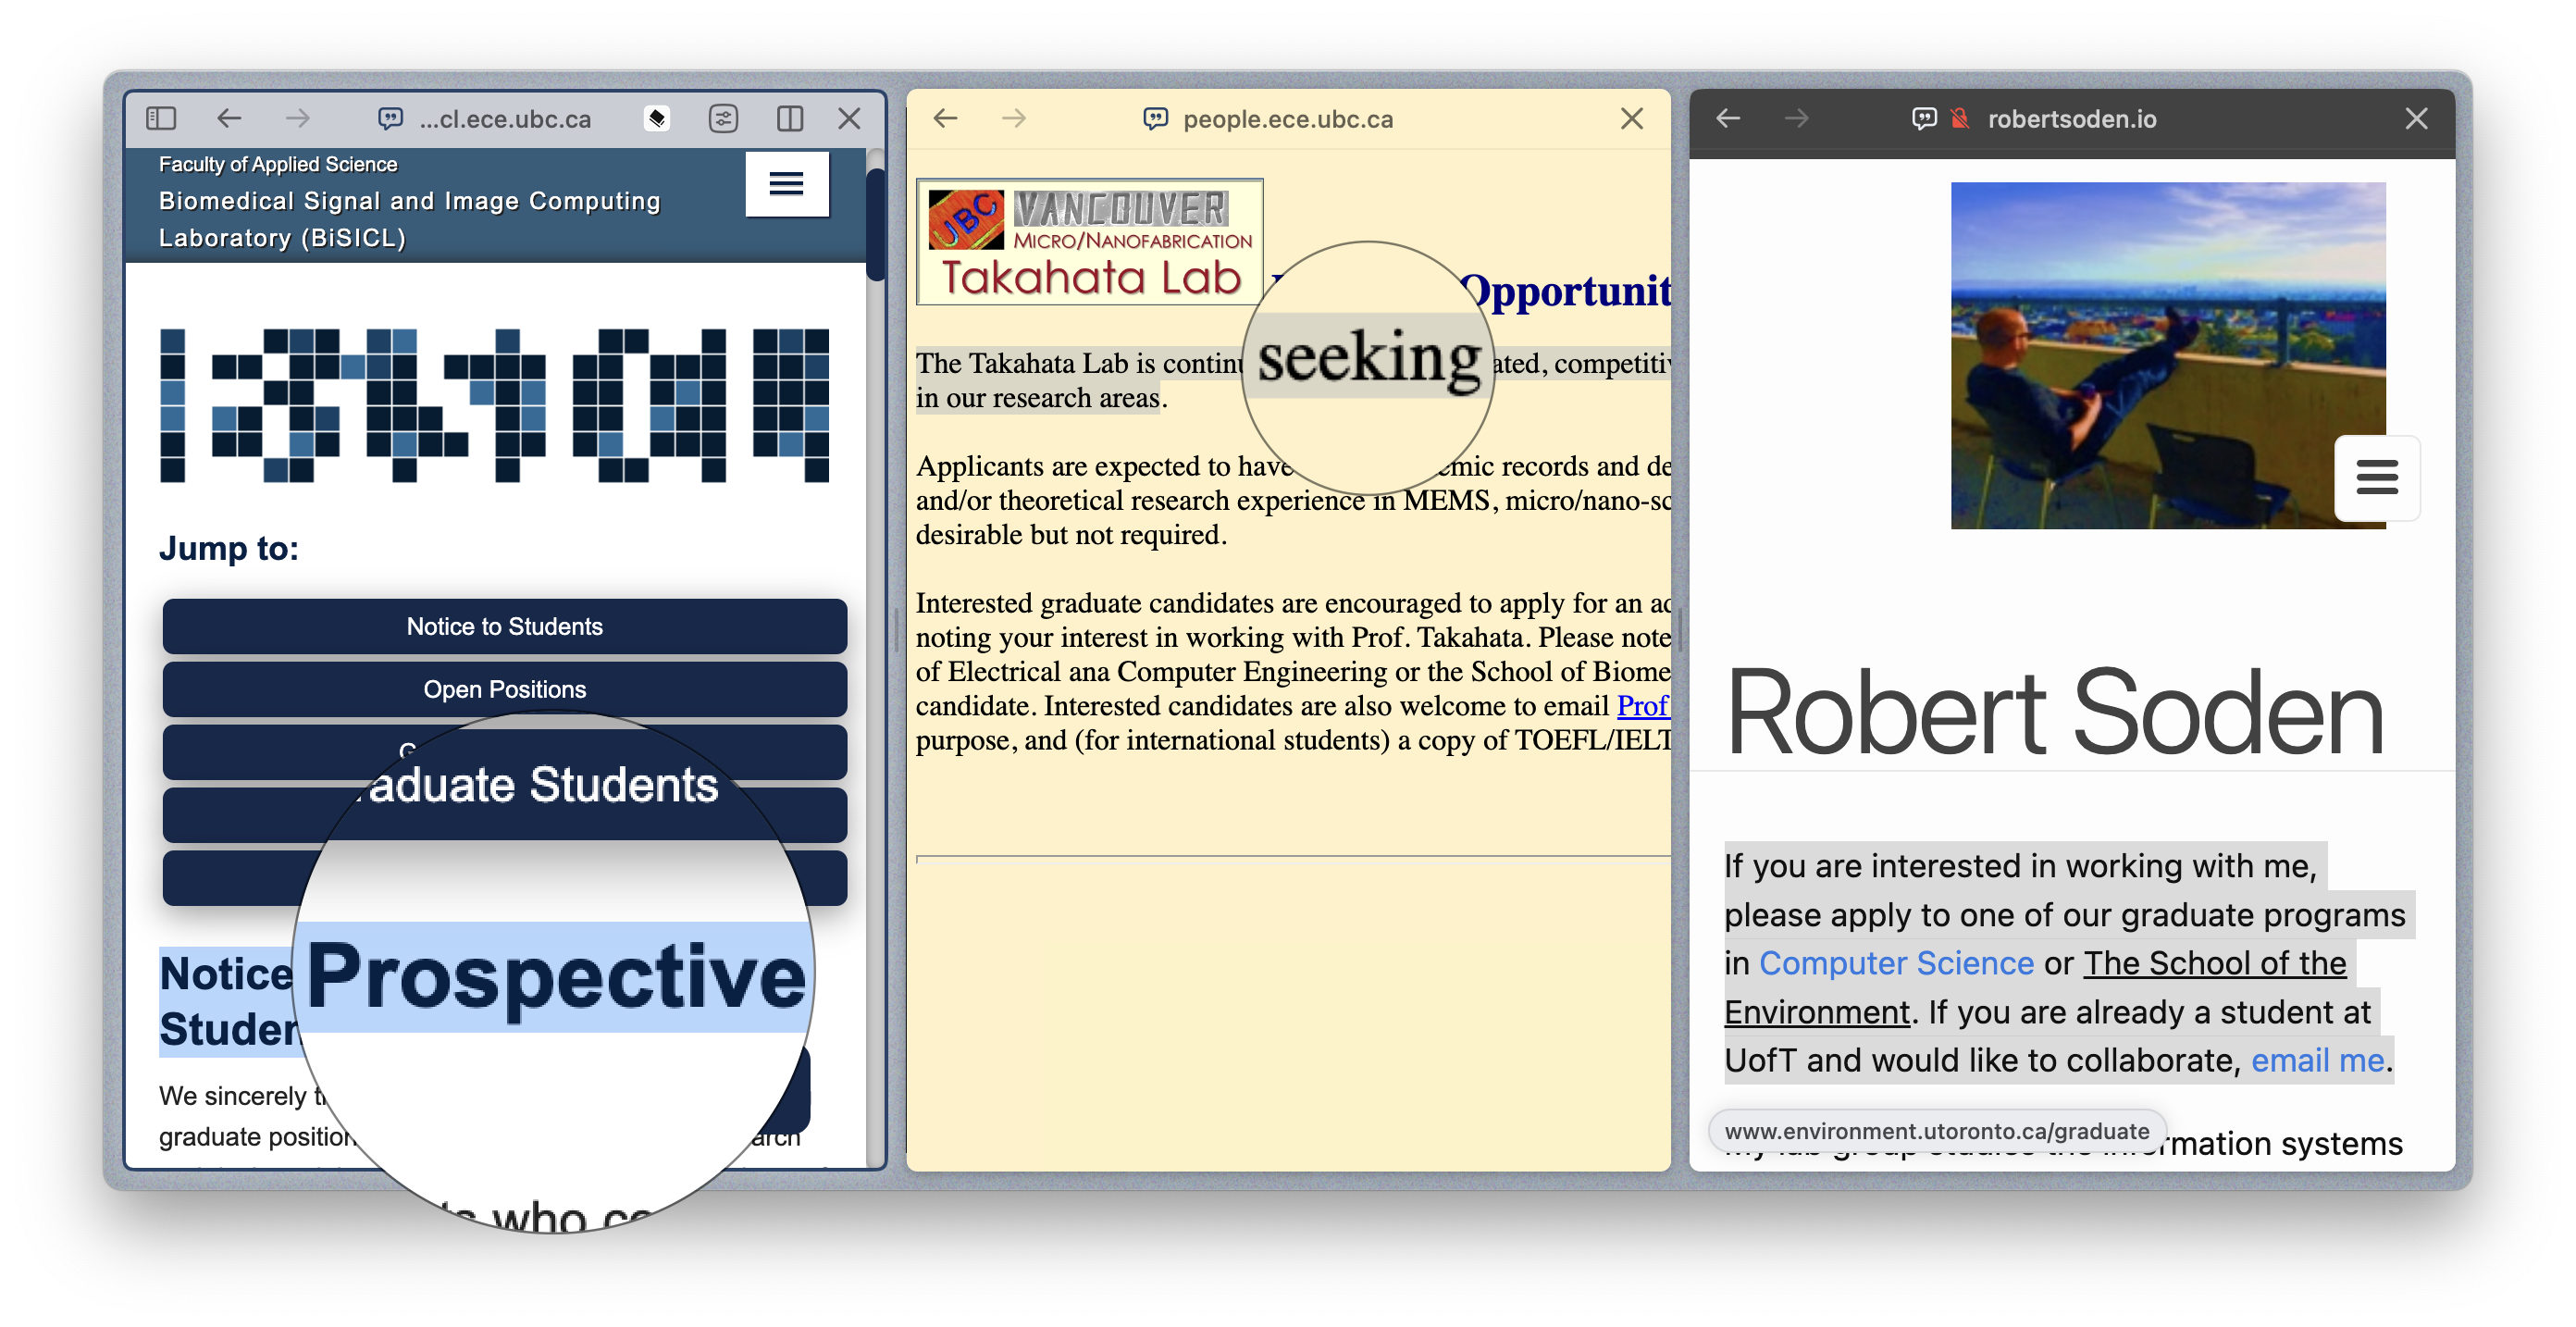
\includegraphics[width=\linewidth]{pic/PotentialSupervisor1.png}
  \end{figure}

\end{frame}

\subsection{Balance}
\begin{frame}{Internship? \hfill Research? \hfill Competitions?}
  \begin{itemize}
    \item Internship: \hfill \emph{Course-based}
    \item Research: \hfill \emph{Research, PhD}
    \item Competitions: \hfill \emph{Course-based, Less Important\footnote{They cannot understand its importance or level}}
  \end{itemize}
\end{frame}

\section{Lookup Table}
\begin{frame}

  \begin{table}[h]
    \centering
    \small
    \begin{tabular}{l|r|r}\toprule

      Abbreviation & Meaning & 中文 \\

      \midrule
      PS & Personal Statement & \\
      SOP & Statement of Purpose & 文书 \\
      SOI & Statement of Interest  & \\
      CV & Curriculum Vitae  & 简历 \\
      RL & Recommendation Letter & 推荐信 \\

      \midrule
      RA & Rolling Admission & 多轮录取\\ 
      WL & Waiting List & 候补\\ 
      AD & Admission & 录取\\ 
      CO & Conditional Offer & 条件录取 \\ 
      COF & Certificate of Finance & 财产证明 \\ 

      \midrule
      BG & Background & 背景情况 \\ 
      Bar & Barrier & 门槛 \\ 
      TL & Timeline  & 时间线\\ 
      GPA & Grade Point Average (4.0) & 成绩\\ 
      RA$^*$ & Research Assistant & 科研助理 \\ 
      \bottomrule
    \end{tabular}
  \end{table}

\end{frame}

\begin{frame}
  \begin{figure}[h]
    \centering
    {Meet you in Singapore :)}\hfill
    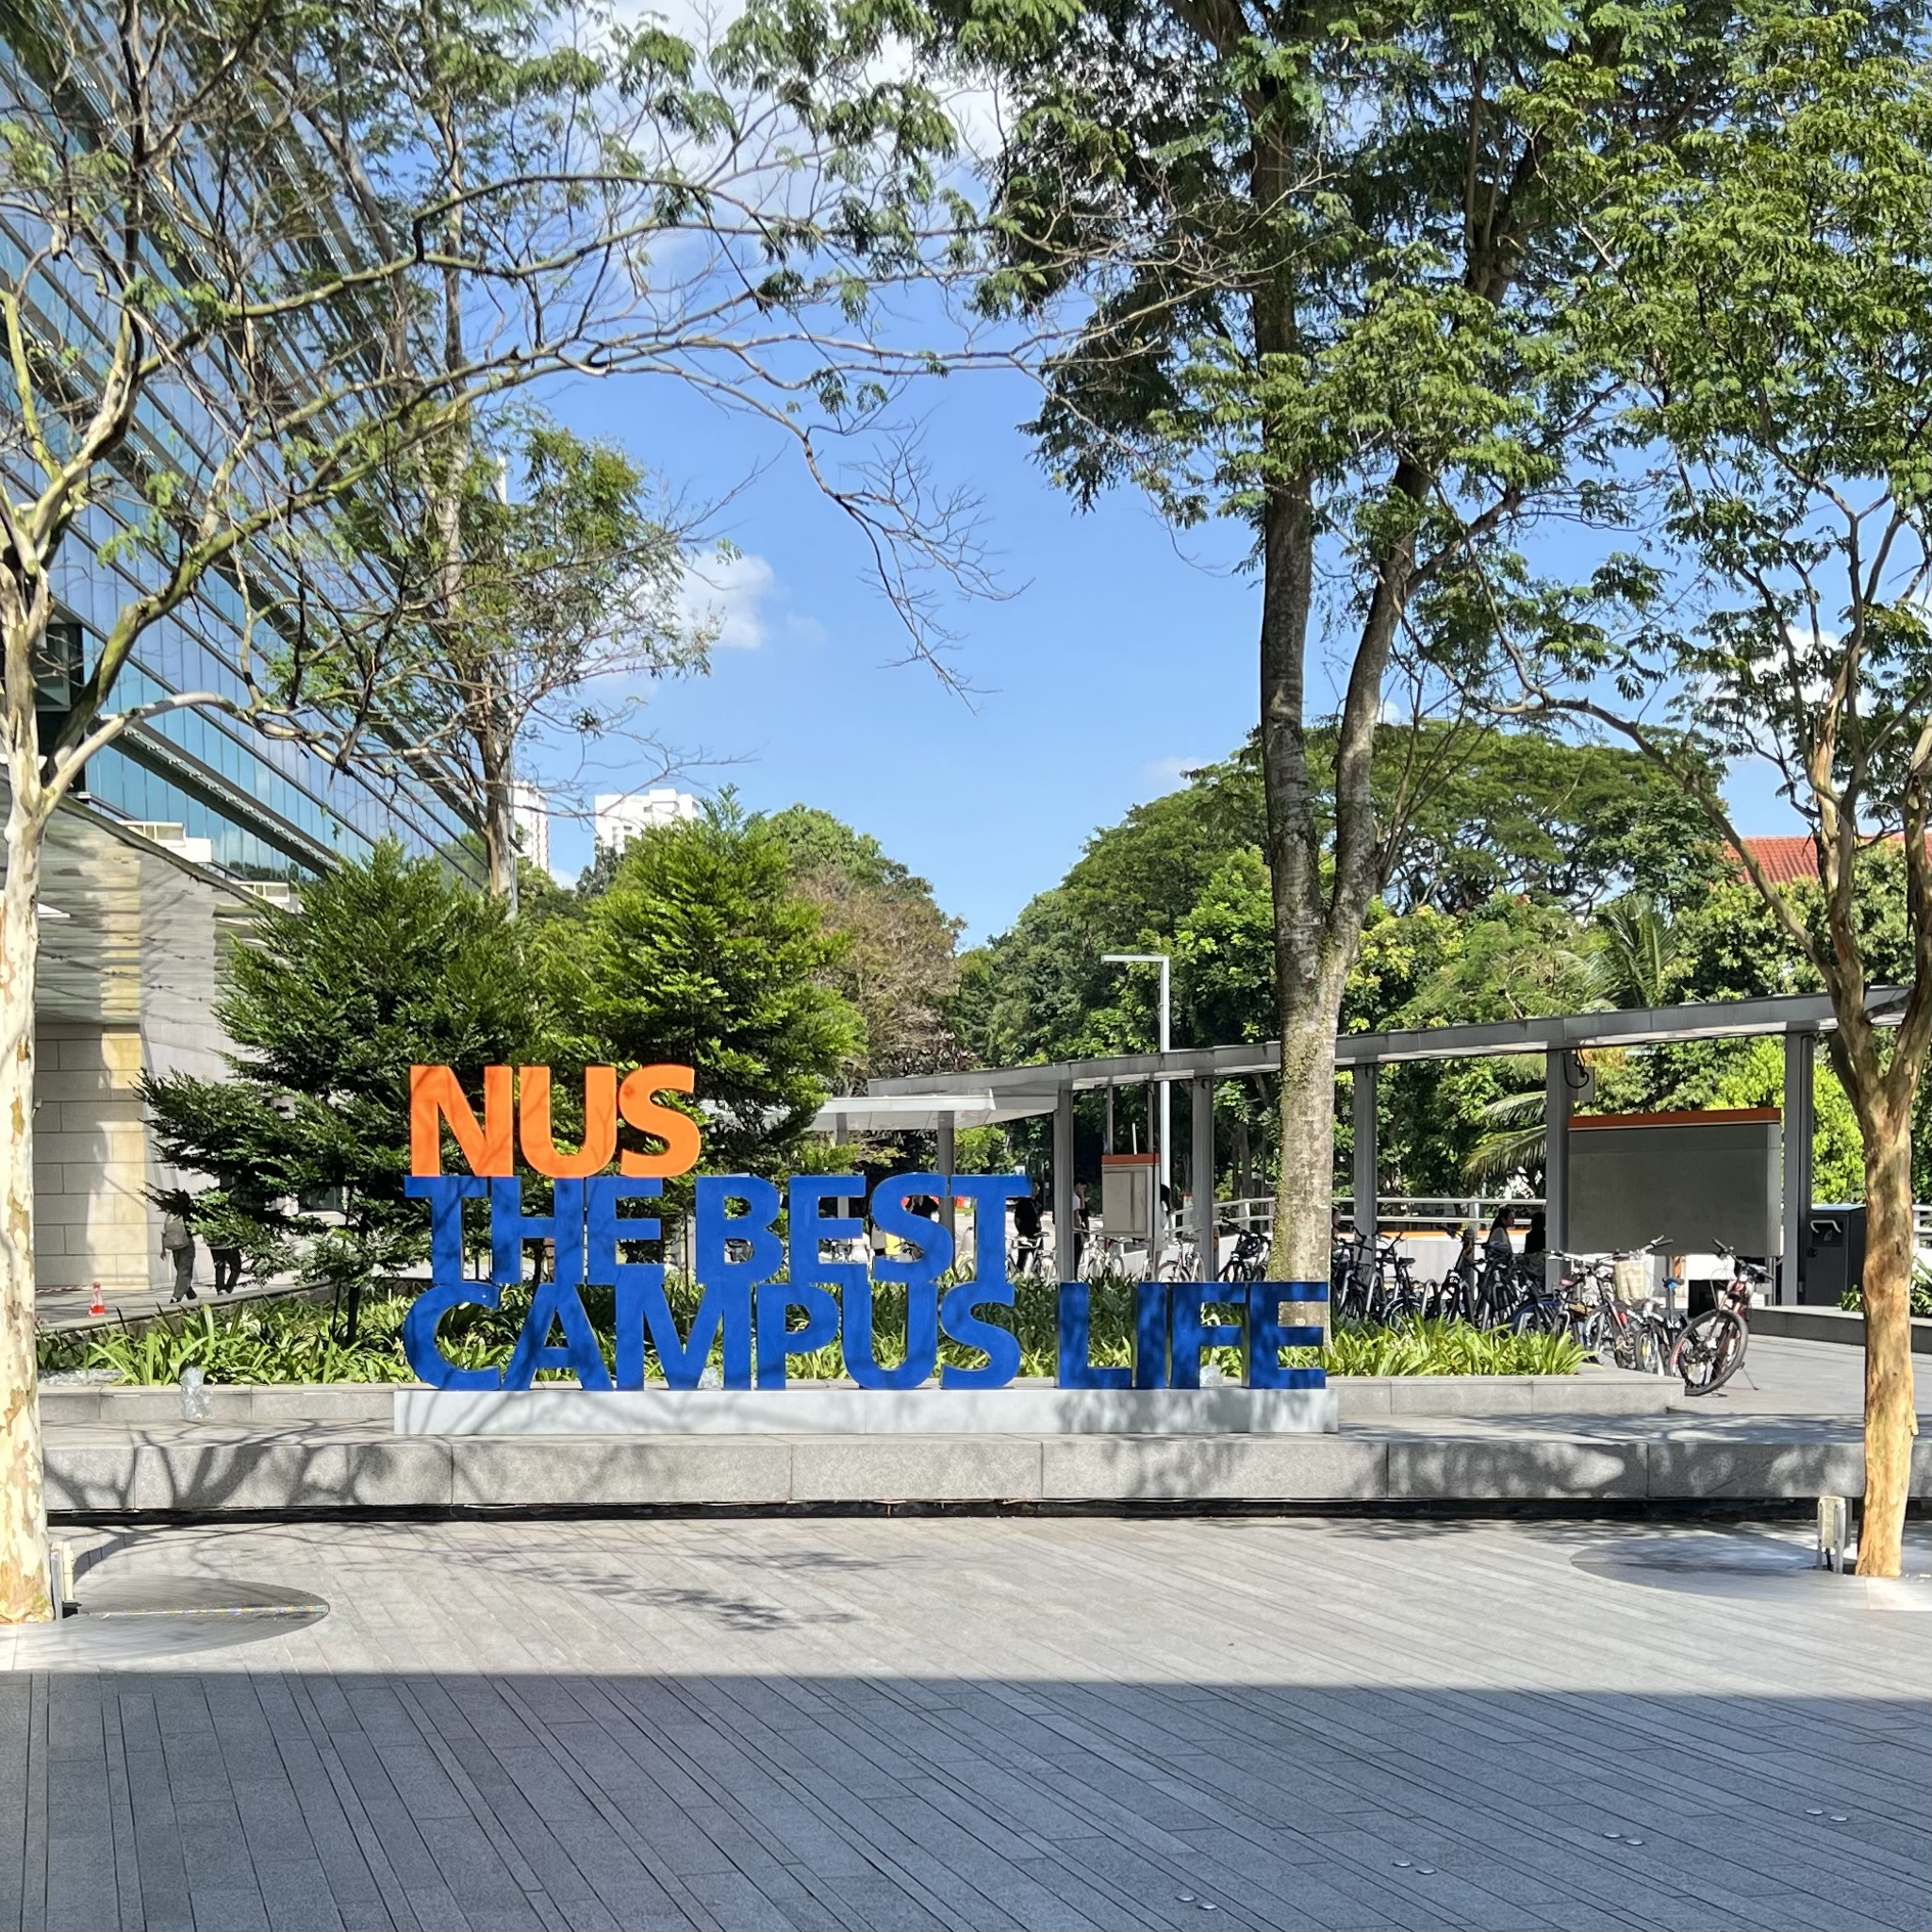
\includegraphics[width=.6\linewidth]{pic/nus.jpeg}
  \end{figure}
\end{frame}
\end{document}
